% \batchmode
% \makeatletter
% \def\input@path{{/Users/nanu/Documents/Projekte/Hydrologie/GavsModel/documentation//}}
% \makeatother
\documentclass[twoside,english]{article}
\usepackage{graphicx, color}
\usepackage{color}%

%============== start knitr Sweave code highlighting declarations ==============

\newcommand{\hlnumber}[1]{\textcolor[rgb]{0,0,0}{#1}}%
\newcommand{\hlfunctioncall}[1]{\textcolor[rgb]{.5,0,.33}{\textbf{#1}}}%
\newcommand{\hlstring}[1]{\textcolor[rgb]{.6,.6,1}{#1}}%
\newcommand{\hlkeyword}[1]{\textbf{#1}}%
\newcommand{\hlargument}[1]{\textcolor[rgb]{.69,.25,.02}{#1}}%
\newcommand{\hlcomment}[1]{\textcolor[rgb]{.18,.6,.34}{#1}}%
\newcommand{\hlroxygencomment}[1]{\textcolor[rgb]{.44,.48,.7}{#1}}%
\newcommand{\hlformalargs}[1]{\hlargument{#1}}%
\newcommand{\hleqformalargs}[1]{\hlargument{#1}}%
\newcommand{\hlassignement}[1]{\textbf{#1}}%
\newcommand{\hlpackage}[1]{\textcolor[rgb]{.59,.71,.145}{#1}}%
\newcommand{\hlslot}[1]{\textit{#1}}%
\newcommand{\hlsymbol}[1]{#1}%
\newcommand{\hlprompt}[1]{\textcolor[rgb]{.5,.5,.5}{#1}}%

 
\newsavebox{\hlnormalsizeboxclosebrace}%
\newsavebox{\hlnormalsizeboxopenbrace}%
\newsavebox{\hlnormalsizeboxbackslash}%
\newsavebox{\hlnormalsizeboxlessthan}%
\newsavebox{\hlnormalsizeboxgreaterthan}%
\newsavebox{\hlnormalsizeboxdollar}%
\newsavebox{\hlnormalsizeboxunderscore}%
\newsavebox{\hlnormalsizeboxand}%
\newsavebox{\hlnormalsizeboxhash}%
\newsavebox{\hlnormalsizeboxat}%
\newsavebox{\hlnormalsizeboxpercent}% 
\newsavebox{\hlnormalsizeboxhat}%
\newsavebox{\hlnormalsizeboxsinglequote}%
\newsavebox{\hlnormalsizeboxbacktick}%

\setbox\hlnormalsizeboxopenbrace=\hbox{\begin{normalsize}\verb.{.\end{normalsize}}%
\setbox\hlnormalsizeboxclosebrace=\hbox{\begin{normalsize}\verb.}.\end{normalsize}}%
\setbox\hlnormalsizeboxlessthan=\hbox{\begin{normalsize}\verb.<.\end{normalsize}}%
\setbox\hlnormalsizeboxdollar=\hbox{\begin{normalsize}\verb.$.\end{normalsize}}%
\setbox\hlnormalsizeboxunderscore=\hbox{\begin{normalsize}\verb._.\end{normalsize}}%
\setbox\hlnormalsizeboxand=\hbox{\begin{normalsize}\verb.&.\end{normalsize}}%
\setbox\hlnormalsizeboxhash=\hbox{\begin{normalsize}\verb.#.\end{normalsize}}%
\setbox\hlnormalsizeboxat=\hbox{\begin{normalsize}\verb.@.\end{normalsize}}%
\setbox\hlnormalsizeboxbackslash=\hbox{\begin{normalsize}\verb.\.\end{normalsize}}%
\setbox\hlnormalsizeboxgreaterthan=\hbox{\begin{normalsize}\verb.>.\end{normalsize}}%
\setbox\hlnormalsizeboxpercent=\hbox{\begin{normalsize}\verb.%.\end{normalsize}}%
\setbox\hlnormalsizeboxhat=\hbox{\begin{normalsize}\verb.^.\end{normalsize}}%
\setbox\hlnormalsizeboxsinglequote=\hbox{\begin{normalsize}\verb.'.\end{normalsize}}%
\setbox\hlnormalsizeboxbacktick=\hbox{\begin{normalsize}\verb.`.\end{normalsize}}%
\setbox\hlnormalsizeboxhat=\hbox{\begin{normalsize}\verb.^.\end{normalsize}}%



\newsavebox{\hltinyboxclosebrace}%
\newsavebox{\hltinyboxopenbrace}%
\newsavebox{\hltinyboxbackslash}%
\newsavebox{\hltinyboxlessthan}%
\newsavebox{\hltinyboxgreaterthan}%
\newsavebox{\hltinyboxdollar}%
\newsavebox{\hltinyboxunderscore}%
\newsavebox{\hltinyboxand}%
\newsavebox{\hltinyboxhash}%
\newsavebox{\hltinyboxat}%
\newsavebox{\hltinyboxpercent}% 
\newsavebox{\hltinyboxhat}%
\newsavebox{\hltinyboxsinglequote}%
\newsavebox{\hltinyboxbacktick}%

\setbox\hltinyboxopenbrace=\hbox{\begin{tiny}\verb.{.\end{tiny}}%
\setbox\hltinyboxclosebrace=\hbox{\begin{tiny}\verb.}.\end{tiny}}%
\setbox\hltinyboxlessthan=\hbox{\begin{tiny}\verb.<.\end{tiny}}%
\setbox\hltinyboxdollar=\hbox{\begin{tiny}\verb.$.\end{tiny}}%
\setbox\hltinyboxunderscore=\hbox{\begin{tiny}\verb._.\end{tiny}}%
\setbox\hltinyboxand=\hbox{\begin{tiny}\verb.&.\end{tiny}}%
\setbox\hltinyboxhash=\hbox{\begin{tiny}\verb.#.\end{tiny}}%
\setbox\hltinyboxat=\hbox{\begin{tiny}\verb.@.\end{tiny}}%
\setbox\hltinyboxbackslash=\hbox{\begin{tiny}\verb.\.\end{tiny}}%
\setbox\hltinyboxgreaterthan=\hbox{\begin{tiny}\verb.>.\end{tiny}}%
\setbox\hltinyboxpercent=\hbox{\begin{tiny}\verb.%.\end{tiny}}%
\setbox\hltinyboxhat=\hbox{\begin{tiny}\verb.^.\end{tiny}}%
\setbox\hltinyboxsinglequote=\hbox{\begin{tiny}\verb.'.\end{tiny}}%
\setbox\hltinyboxbacktick=\hbox{\begin{tiny}\verb.`.\end{tiny}}%
\setbox\hltinyboxhat=\hbox{\begin{tiny}\verb.^.\end{tiny}}%



\newsavebox{\hlscriptsizeboxclosebrace}%
\newsavebox{\hlscriptsizeboxopenbrace}%
\newsavebox{\hlscriptsizeboxbackslash}%
\newsavebox{\hlscriptsizeboxlessthan}%
\newsavebox{\hlscriptsizeboxgreaterthan}%
\newsavebox{\hlscriptsizeboxdollar}%
\newsavebox{\hlscriptsizeboxunderscore}%
\newsavebox{\hlscriptsizeboxand}%
\newsavebox{\hlscriptsizeboxhash}%
\newsavebox{\hlscriptsizeboxat}%
\newsavebox{\hlscriptsizeboxpercent}% 
\newsavebox{\hlscriptsizeboxhat}%
\newsavebox{\hlscriptsizeboxsinglequote}%
\newsavebox{\hlscriptsizeboxbacktick}%

\setbox\hlscriptsizeboxopenbrace=\hbox{\begin{scriptsize}\verb.{.\end{scriptsize}}%
\setbox\hlscriptsizeboxclosebrace=\hbox{\begin{scriptsize}\verb.}.\end{scriptsize}}%
\setbox\hlscriptsizeboxlessthan=\hbox{\begin{scriptsize}\verb.<.\end{scriptsize}}%
\setbox\hlscriptsizeboxdollar=\hbox{\begin{scriptsize}\verb.$.\end{scriptsize}}%
\setbox\hlscriptsizeboxunderscore=\hbox{\begin{scriptsize}\verb._.\end{scriptsize}}%
\setbox\hlscriptsizeboxand=\hbox{\begin{scriptsize}\verb.&.\end{scriptsize}}%
\setbox\hlscriptsizeboxhash=\hbox{\begin{scriptsize}\verb.#.\end{scriptsize}}%
\setbox\hlscriptsizeboxat=\hbox{\begin{scriptsize}\verb.@.\end{scriptsize}}%
\setbox\hlscriptsizeboxbackslash=\hbox{\begin{scriptsize}\verb.\.\end{scriptsize}}%
\setbox\hlscriptsizeboxgreaterthan=\hbox{\begin{scriptsize}\verb.>.\end{scriptsize}}%
\setbox\hlscriptsizeboxpercent=\hbox{\begin{scriptsize}\verb.%.\end{scriptsize}}%
\setbox\hlscriptsizeboxhat=\hbox{\begin{scriptsize}\verb.^.\end{scriptsize}}%
\setbox\hlscriptsizeboxsinglequote=\hbox{\begin{scriptsize}\verb.'.\end{scriptsize}}%
\setbox\hlscriptsizeboxbacktick=\hbox{\begin{scriptsize}\verb.`.\end{scriptsize}}%
\setbox\hlscriptsizeboxhat=\hbox{\begin{scriptsize}\verb.^.\end{scriptsize}}%



\newsavebox{\hlfootnotesizeboxclosebrace}%
\newsavebox{\hlfootnotesizeboxopenbrace}%
\newsavebox{\hlfootnotesizeboxbackslash}%
\newsavebox{\hlfootnotesizeboxlessthan}%
\newsavebox{\hlfootnotesizeboxgreaterthan}%
\newsavebox{\hlfootnotesizeboxdollar}%
\newsavebox{\hlfootnotesizeboxunderscore}%
\newsavebox{\hlfootnotesizeboxand}%
\newsavebox{\hlfootnotesizeboxhash}%
\newsavebox{\hlfootnotesizeboxat}%
\newsavebox{\hlfootnotesizeboxpercent}% 
\newsavebox{\hlfootnotesizeboxhat}%
\newsavebox{\hlfootnotesizeboxsinglequote}%
\newsavebox{\hlfootnotesizeboxbacktick}%

\setbox\hlfootnotesizeboxopenbrace=\hbox{\begin{footnotesize}\verb.{.\end{footnotesize}}%
\setbox\hlfootnotesizeboxclosebrace=\hbox{\begin{footnotesize}\verb.}.\end{footnotesize}}%
\setbox\hlfootnotesizeboxlessthan=\hbox{\begin{footnotesize}\verb.<.\end{footnotesize}}%
\setbox\hlfootnotesizeboxdollar=\hbox{\begin{footnotesize}\verb.$.\end{footnotesize}}%
\setbox\hlfootnotesizeboxunderscore=\hbox{\begin{footnotesize}\verb._.\end{footnotesize}}%
\setbox\hlfootnotesizeboxand=\hbox{\begin{footnotesize}\verb.&.\end{footnotesize}}%
\setbox\hlfootnotesizeboxhash=\hbox{\begin{footnotesize}\verb.#.\end{footnotesize}}%
\setbox\hlfootnotesizeboxat=\hbox{\begin{footnotesize}\verb.@.\end{footnotesize}}%
\setbox\hlfootnotesizeboxbackslash=\hbox{\begin{footnotesize}\verb.\.\end{footnotesize}}%
\setbox\hlfootnotesizeboxgreaterthan=\hbox{\begin{footnotesize}\verb.>.\end{footnotesize}}%
\setbox\hlfootnotesizeboxpercent=\hbox{\begin{footnotesize}\verb.%.\end{footnotesize}}%
\setbox\hlfootnotesizeboxhat=\hbox{\begin{footnotesize}\verb.^.\end{footnotesize}}%
\setbox\hlfootnotesizeboxsinglequote=\hbox{\begin{footnotesize}\verb.'.\end{footnotesize}}%
\setbox\hlfootnotesizeboxbacktick=\hbox{\begin{footnotesize}\verb.`.\end{footnotesize}}%
\setbox\hlfootnotesizeboxhat=\hbox{\begin{footnotesize}\verb.^.\end{footnotesize}}%



\newsavebox{\hlsmallboxclosebrace}%
\newsavebox{\hlsmallboxopenbrace}%
\newsavebox{\hlsmallboxbackslash}%
\newsavebox{\hlsmallboxlessthan}%
\newsavebox{\hlsmallboxgreaterthan}%
\newsavebox{\hlsmallboxdollar}%
\newsavebox{\hlsmallboxunderscore}%
\newsavebox{\hlsmallboxand}%
\newsavebox{\hlsmallboxhash}%
\newsavebox{\hlsmallboxat}%
\newsavebox{\hlsmallboxpercent}% 
\newsavebox{\hlsmallboxhat}%
\newsavebox{\hlsmallboxsinglequote}%
\newsavebox{\hlsmallboxbacktick}%

\setbox\hlsmallboxopenbrace=\hbox{\begin{small}\verb.{.\end{small}}%
\setbox\hlsmallboxclosebrace=\hbox{\begin{small}\verb.}.\end{small}}%
\setbox\hlsmallboxlessthan=\hbox{\begin{small}\verb.<.\end{small}}%
\setbox\hlsmallboxdollar=\hbox{\begin{small}\verb.$.\end{small}}%
\setbox\hlsmallboxunderscore=\hbox{\begin{small}\verb._.\end{small}}%
\setbox\hlsmallboxand=\hbox{\begin{small}\verb.&.\end{small}}%
\setbox\hlsmallboxhash=\hbox{\begin{small}\verb.#.\end{small}}%
\setbox\hlsmallboxat=\hbox{\begin{small}\verb.@.\end{small}}%
\setbox\hlsmallboxbackslash=\hbox{\begin{small}\verb.\.\end{small}}%
\setbox\hlsmallboxgreaterthan=\hbox{\begin{small}\verb.>.\end{small}}%
\setbox\hlsmallboxpercent=\hbox{\begin{small}\verb.%.\end{small}}%
\setbox\hlsmallboxhat=\hbox{\begin{small}\verb.^.\end{small}}%
\setbox\hlsmallboxsinglequote=\hbox{\begin{small}\verb.'.\end{small}}%
\setbox\hlsmallboxbacktick=\hbox{\begin{small}\verb.`.\end{small}}%
\setbox\hlsmallboxhat=\hbox{\begin{small}\verb.^.\end{small}}%



\newsavebox{\hllargeboxclosebrace}%
\newsavebox{\hllargeboxopenbrace}%
\newsavebox{\hllargeboxbackslash}%
\newsavebox{\hllargeboxlessthan}%
\newsavebox{\hllargeboxgreaterthan}%
\newsavebox{\hllargeboxdollar}%
\newsavebox{\hllargeboxunderscore}%
\newsavebox{\hllargeboxand}%
\newsavebox{\hllargeboxhash}%
\newsavebox{\hllargeboxat}%
\newsavebox{\hllargeboxpercent}% 
\newsavebox{\hllargeboxhat}%
\newsavebox{\hllargeboxsinglequote}%
\newsavebox{\hllargeboxbacktick}%

\setbox\hllargeboxopenbrace=\hbox{\begin{large}\verb.{.\end{large}}%
\setbox\hllargeboxclosebrace=\hbox{\begin{large}\verb.}.\end{large}}%
\setbox\hllargeboxlessthan=\hbox{\begin{large}\verb.<.\end{large}}%
\setbox\hllargeboxdollar=\hbox{\begin{large}\verb.$.\end{large}}%
\setbox\hllargeboxunderscore=\hbox{\begin{large}\verb._.\end{large}}%
\setbox\hllargeboxand=\hbox{\begin{large}\verb.&.\end{large}}%
\setbox\hllargeboxhash=\hbox{\begin{large}\verb.#.\end{large}}%
\setbox\hllargeboxat=\hbox{\begin{large}\verb.@.\end{large}}%
\setbox\hllargeboxbackslash=\hbox{\begin{large}\verb.\.\end{large}}%
\setbox\hllargeboxgreaterthan=\hbox{\begin{large}\verb.>.\end{large}}%
\setbox\hllargeboxpercent=\hbox{\begin{large}\verb.%.\end{large}}%
\setbox\hllargeboxhat=\hbox{\begin{large}\verb.^.\end{large}}%
\setbox\hllargeboxsinglequote=\hbox{\begin{large}\verb.'.\end{large}}%
\setbox\hllargeboxbacktick=\hbox{\begin{large}\verb.`.\end{large}}%
\setbox\hllargeboxhat=\hbox{\begin{large}\verb.^.\end{large}}%



\newsavebox{\hlLargeboxclosebrace}%
\newsavebox{\hlLargeboxopenbrace}%
\newsavebox{\hlLargeboxbackslash}%
\newsavebox{\hlLargeboxlessthan}%
\newsavebox{\hlLargeboxgreaterthan}%
\newsavebox{\hlLargeboxdollar}%
\newsavebox{\hlLargeboxunderscore}%
\newsavebox{\hlLargeboxand}%
\newsavebox{\hlLargeboxhash}%
\newsavebox{\hlLargeboxat}%
\newsavebox{\hlLargeboxpercent}% 
\newsavebox{\hlLargeboxhat}%
\newsavebox{\hlLargeboxsinglequote}%
\newsavebox{\hlLargeboxbacktick}%

\setbox\hlLargeboxopenbrace=\hbox{\begin{Large}\verb.{.\end{Large}}%
\setbox\hlLargeboxclosebrace=\hbox{\begin{Large}\verb.}.\end{Large}}%
\setbox\hlLargeboxlessthan=\hbox{\begin{Large}\verb.<.\end{Large}}%
\setbox\hlLargeboxdollar=\hbox{\begin{Large}\verb.$.\end{Large}}%
\setbox\hlLargeboxunderscore=\hbox{\begin{Large}\verb._.\end{Large}}%
\setbox\hlLargeboxand=\hbox{\begin{Large}\verb.&.\end{Large}}%
\setbox\hlLargeboxhash=\hbox{\begin{Large}\verb.#.\end{Large}}%
\setbox\hlLargeboxat=\hbox{\begin{Large}\verb.@.\end{Large}}%
\setbox\hlLargeboxbackslash=\hbox{\begin{Large}\verb.\.\end{Large}}%
\setbox\hlLargeboxgreaterthan=\hbox{\begin{Large}\verb.>.\end{Large}}%
\setbox\hlLargeboxpercent=\hbox{\begin{Large}\verb.%.\end{Large}}%
\setbox\hlLargeboxhat=\hbox{\begin{Large}\verb.^.\end{Large}}%
\setbox\hlLargeboxsinglequote=\hbox{\begin{Large}\verb.'.\end{Large}}%
\setbox\hlLargeboxbacktick=\hbox{\begin{Large}\verb.`.\end{Large}}%
\setbox\hlLargeboxhat=\hbox{\begin{Large}\verb.^.\end{Large}}%



\newsavebox{\hlLARGEboxclosebrace}%
\newsavebox{\hlLARGEboxopenbrace}%
\newsavebox{\hlLARGEboxbackslash}%
\newsavebox{\hlLARGEboxlessthan}%
\newsavebox{\hlLARGEboxgreaterthan}%
\newsavebox{\hlLARGEboxdollar}%
\newsavebox{\hlLARGEboxunderscore}%
\newsavebox{\hlLARGEboxand}%
\newsavebox{\hlLARGEboxhash}%
\newsavebox{\hlLARGEboxat}%
\newsavebox{\hlLARGEboxpercent}% 
\newsavebox{\hlLARGEboxhat}%
\newsavebox{\hlLARGEboxsinglequote}%
\newsavebox{\hlLARGEboxbacktick}%

\setbox\hlLARGEboxopenbrace=\hbox{\begin{LARGE}\verb.{.\end{LARGE}}%
\setbox\hlLARGEboxclosebrace=\hbox{\begin{LARGE}\verb.}.\end{LARGE}}%
\setbox\hlLARGEboxlessthan=\hbox{\begin{LARGE}\verb.<.\end{LARGE}}%
\setbox\hlLARGEboxdollar=\hbox{\begin{LARGE}\verb.$.\end{LARGE}}%
\setbox\hlLARGEboxunderscore=\hbox{\begin{LARGE}\verb._.\end{LARGE}}%
\setbox\hlLARGEboxand=\hbox{\begin{LARGE}\verb.&.\end{LARGE}}%
\setbox\hlLARGEboxhash=\hbox{\begin{LARGE}\verb.#.\end{LARGE}}%
\setbox\hlLARGEboxat=\hbox{\begin{LARGE}\verb.@.\end{LARGE}}%
\setbox\hlLARGEboxbackslash=\hbox{\begin{LARGE}\verb.\.\end{LARGE}}%
\setbox\hlLARGEboxgreaterthan=\hbox{\begin{LARGE}\verb.>.\end{LARGE}}%
\setbox\hlLARGEboxpercent=\hbox{\begin{LARGE}\verb.%.\end{LARGE}}%
\setbox\hlLARGEboxhat=\hbox{\begin{LARGE}\verb.^.\end{LARGE}}%
\setbox\hlLARGEboxsinglequote=\hbox{\begin{LARGE}\verb.'.\end{LARGE}}%
\setbox\hlLARGEboxbacktick=\hbox{\begin{LARGE}\verb.`.\end{LARGE}}%
\setbox\hlLARGEboxhat=\hbox{\begin{LARGE}\verb.^.\end{LARGE}}%



\newsavebox{\hlhugeboxclosebrace}%
\newsavebox{\hlhugeboxopenbrace}%
\newsavebox{\hlhugeboxbackslash}%
\newsavebox{\hlhugeboxlessthan}%
\newsavebox{\hlhugeboxgreaterthan}%
\newsavebox{\hlhugeboxdollar}%
\newsavebox{\hlhugeboxunderscore}%
\newsavebox{\hlhugeboxand}%
\newsavebox{\hlhugeboxhash}%
\newsavebox{\hlhugeboxat}%
\newsavebox{\hlhugeboxpercent}% 
\newsavebox{\hlhugeboxhat}%
\newsavebox{\hlhugeboxsinglequote}%
\newsavebox{\hlhugeboxbacktick}%

\setbox\hlhugeboxopenbrace=\hbox{\begin{huge}\verb.{.\end{huge}}%
\setbox\hlhugeboxclosebrace=\hbox{\begin{huge}\verb.}.\end{huge}}%
\setbox\hlhugeboxlessthan=\hbox{\begin{huge}\verb.<.\end{huge}}%
\setbox\hlhugeboxdollar=\hbox{\begin{huge}\verb.$.\end{huge}}%
\setbox\hlhugeboxunderscore=\hbox{\begin{huge}\verb._.\end{huge}}%
\setbox\hlhugeboxand=\hbox{\begin{huge}\verb.&.\end{huge}}%
\setbox\hlhugeboxhash=\hbox{\begin{huge}\verb.#.\end{huge}}%
\setbox\hlhugeboxat=\hbox{\begin{huge}\verb.@.\end{huge}}%
\setbox\hlhugeboxbackslash=\hbox{\begin{huge}\verb.\.\end{huge}}%
\setbox\hlhugeboxgreaterthan=\hbox{\begin{huge}\verb.>.\end{huge}}%
\setbox\hlhugeboxpercent=\hbox{\begin{huge}\verb.%.\end{huge}}%
\setbox\hlhugeboxhat=\hbox{\begin{huge}\verb.^.\end{huge}}%
\setbox\hlhugeboxsinglequote=\hbox{\begin{huge}\verb.'.\end{huge}}%
\setbox\hlhugeboxbacktick=\hbox{\begin{huge}\verb.`.\end{huge}}%
\setbox\hlhugeboxhat=\hbox{\begin{huge}\verb.^.\end{huge}}%



\newsavebox{\hlHugeboxclosebrace}%
\newsavebox{\hlHugeboxopenbrace}%
\newsavebox{\hlHugeboxbackslash}%
\newsavebox{\hlHugeboxlessthan}%
\newsavebox{\hlHugeboxgreaterthan}%
\newsavebox{\hlHugeboxdollar}%
\newsavebox{\hlHugeboxunderscore}%
\newsavebox{\hlHugeboxand}%
\newsavebox{\hlHugeboxhash}%
\newsavebox{\hlHugeboxat}%
\newsavebox{\hlHugeboxpercent}% 
\newsavebox{\hlHugeboxhat}%
\newsavebox{\hlHugeboxsinglequote}%
\newsavebox{\hlHugeboxbacktick}%

\setbox\hlHugeboxopenbrace=\hbox{\begin{Huge}\verb.{.\end{Huge}}%
\setbox\hlHugeboxclosebrace=\hbox{\begin{Huge}\verb.}.\end{Huge}}%
\setbox\hlHugeboxlessthan=\hbox{\begin{Huge}\verb.<.\end{Huge}}%
\setbox\hlHugeboxdollar=\hbox{\begin{Huge}\verb.$.\end{Huge}}%
\setbox\hlHugeboxunderscore=\hbox{\begin{Huge}\verb._.\end{Huge}}%
\setbox\hlHugeboxand=\hbox{\begin{Huge}\verb.&.\end{Huge}}%
\setbox\hlHugeboxhash=\hbox{\begin{Huge}\verb.#.\end{Huge}}%
\setbox\hlHugeboxat=\hbox{\begin{Huge}\verb.@.\end{Huge}}%
\setbox\hlHugeboxbackslash=\hbox{\begin{Huge}\verb.\.\end{Huge}}%
\setbox\hlHugeboxgreaterthan=\hbox{\begin{Huge}\verb.>.\end{Huge}}%
\setbox\hlHugeboxpercent=\hbox{\begin{Huge}\verb.%.\end{Huge}}%
\setbox\hlHugeboxhat=\hbox{\begin{Huge}\verb.^.\end{Huge}}%
\setbox\hlHugeboxsinglequote=\hbox{\begin{Huge}\verb.'.\end{Huge}}%
\setbox\hlHugeboxbacktick=\hbox{\begin{Huge}\verb.`.\end{Huge}}%
\setbox\hlHugeboxhat=\hbox{\begin{Huge}\verb.^.\end{Huge}}%
 

\def\urltilda{\kern -.15em\lower .7ex\hbox{\~{}}\kern .04em}%

\newcommand{\hlstd}[1]{\textcolor[rgb]{0,0,0}{#1}}%
\newcommand{\hlnum}[1]{\textcolor[rgb]{0.16,0.16,1}{#1}}
\newcommand{\hlesc}[1]{\textcolor[rgb]{1,0,1}{#1}}
\newcommand{\hlstr}[1]{\textcolor[rgb]{1,0,0}{#1}}
\newcommand{\hldstr}[1]{\textcolor[rgb]{0.51,0.51,0}{#1}}
\newcommand{\hlslc}[1]{\textcolor[rgb]{0.51,0.51,0.51}{\it{#1}}}
\newcommand{\hlcom}[1]{\textcolor[rgb]{0.51,0.51,0.51}{\it{#1}}}
\newcommand{\hldir}[1]{\textcolor[rgb]{0,0.51,0}{#1}}
\newcommand{\hlsym}[1]{\textcolor[rgb]{0,0,0}{#1}}
\newcommand{\hlline}[1]{\textcolor[rgb]{0.33,0.33,0.33}{#1}}
\newcommand{\hlkwa}[1]{\textcolor[rgb]{0,0,0}{\bf{#1}}}
\newcommand{\hlkwb}[1]{\textcolor[rgb]{0.51,0,0}{#1}}
\newcommand{\hlkwc}[1]{\textcolor[rgb]{0,0,0}{\bf{#1}}}
\newcommand{\hlkwd}[1]{\textcolor[rgb]{0,0,0.51}{#1}}

\definecolor{fgcolor}{rgb}{0,0,0}
\usepackage{framed}
\makeatletter
\newenvironment{kframe}{%
 \def\FrameCommand##1{\hskip\@totalleftmargin \hskip-\fboxsep
 \colorbox{shadecolor}{##1}\hskip-\fboxsep
     % There is no \@totalrightmargin, so:
     \hskip-\linewidth \hskip-\@totalleftmargin \hskip\columnwidth}%
 \MakeFramed {\advance\hsize-\width
   \@totalleftmargin\z@ \linewidth\hsize
   \@setminipage}}%
 {\par\unskip\endMakeFramed}
\makeatother

\definecolor{shadecolor}{rgb}{.97, .97, .97}
\newenvironment{knitrout}{}{} % an empty environment to be redefined in TeX

\newcommand{\SweaveOpts}[1]{}  % do not interfere with LaTeX
\newcommand{\SweaveInput}[1]{} % because they are not real TeX commands
\newcommand{\Sexpr}[1]{}       % will only be parsed by R

%============== end knitr Sweave ==============

\renewcommand{\sfdefault}{cmbr}
\usepackage{courier}
\renewcommand{\familydefault}{\sfdefault}
\usepackage[T1]{fontenc}
\usepackage[latin9]{inputenc}

% Package for insertion of Code examples with highlighting
\usepackage{listings}
\lstset{basicstyle={\ttfamily},
breaklines=true,
escapeinside={(*}{*)},
float,
frame=single,
language={[90]Fortran},
numbers=left,
numberstyle={\small},
tabsize=4}

% page format
\usepackage[a4paper]{geometry}
% page margins
\geometry{verbose,tmargin=2cm,bmargin=2cm,lmargin=3cm,rmargin=2cm}

% for headers:
\usepackage{fancyhdr}
\pagestyle{fancy}
\setlength{\parskip}{\bigskipamount}
\setlength{\parindent}{0pt}
\synctex=1

\usepackage{babel}
\usepackage{array}
\usepackage{float}
\usepackage{units} % for \unit{} and \unitfrac{}{} in formula
\usepackage{amsmath}
\usepackage{amssymb}
\usepackage{tabulary}

% for keyword index:
\usepackage{makeidx} 
\makeindex

\usepackage{graphicx}
\usepackage[authoryear]{natbib}

% for nomenclature:
\usepackage{nomencl}
% the following is useful when we have the old nomencl.sty package
\providecommand{\printnomenclature}{\printglossary}
\providecommand{\makenomenclature}{\makeglossary}
\makenomenclature

% for cross links and hyperlinks in pdf:
\usepackage[unicode=true,pdfusetitle,
 bookmarks=true,bookmarksnumbered=true,bookmarksopen=true,bookmarksopenlevel=3,
 breaklinks=true,pdfborder={0 0 0},backref=false,colorlinks=false]
 {hyperref}

\makeatletter

%%%%%%%%%%%%%%%%%%%%%%%%%%%%%% LyX specific LaTeX commands.
% \providecommand{\LyX}{\texorpdfstring%
%   {L\kern-.1667em\lower.25em\hbox{Y}\kern-.125emX\@}
%   {LyX}}
% %% Because html converters don't know tabularnewline
% \providecommand{\tabularnewline}{\\}

\renewcommand{\section}{\@startsection
{section}%                   % the name
{1}%                         % the level
{-6mm}%                       % the indent
{-\baselineskip}%            % the before skip
{0.5\baselineskip}%          % the after skip
{\normalfont\Large\textbf}} % the style

\renewcommand{\subsubsection}{\@startsection
{subsubsection}%                   % the name
{3}%                         % the level
{-6mm}%                       % the indent
{-\baselineskip}%            % the before skip
{0.1\baselineskip}%          % the after skip
{\normalfont\textbf}} % the style

\renewcommand{\subsection}{\@startsection
{subsection}%                   % the name
{2}%                         % the level
{-6mm}%                       % the indent
{-\baselineskip}%            % the before skip
{0.5\baselineskip}%          % the after skip
{\normalfont\large\textbf}} % the style

%\renewcommand{\lstlistingname }{Code snippet}

\usepackage[nodayofweek]{datetime}

%nomenclature in LOC
\def\nompreamble{\addcontentsline{toc}{section}{\nomname}\markboth{\nomname}{\nomname}}

%\usepackage{pdfsync} % for forward and back links between .tex-file and pdf

%For annotations:
\usepackage[inline]{trackchanges}
\addeditor{Chr.}
\addeditor{Gavan}
\addeditor{Nanu}


% \usepackage{mVersion}
% \setVersion{0.1}
% \increaseBuild 

%%%%%%%%%%% input-output description for subroutines %%%%%%%%%%%%%

% needs \usepackage{xifthen} in the preamble
\RequirePackage{xifthen}

\newcommand{\inoutentry}[5][]{% #1 (optional) emphasized index entry? #2 variable name, #3 variable type, #4 dimensions, #5 description
    \hspace*{0.3cm}&\texttt{#2}%
    \ifthenelse{\equal{#1}{emph}}% use bf to myke an amphasized index entry
        {\index{#2@\texttt{#2}|textbf}}%
        {\ifthenelse{\equal{#1}{none}}%
            {}%
            {\index{#2@\texttt{#2}}}%
        }%
    & \hspace*{.5em}{[}#3{]} & \hspace*{.5em}%
        \ifthenelse{\isempty{#4}}%
            {}%
            {{[}#4{]}}%
        \hspace*{.5em} &  #5 \tabularnewline
}

\newcommand{\inout}[2]{     % #1 input, #2 output
    \setlength{\tabcolsep}{0pt}
    \renewcommand{\arraystretch}{1.2}
    \begin{tabulary}{\textwidth}{llllL}
        \multicolumn{2}{l}{\textbf{input}} & & & \\
        \ifthenelse{\isempty{#1}}%
            {\hspace*{0.3cm}&no input\\}
            {#1}
        \noalign{\vskip 2ex}
        \multicolumn{2}{l}{\textbf{output}} & & & \\
        \ifthenelse{\isempty{#2}}%
            {\hspace*{0.3cm}&no output\\}
            {#2}
    \end{tabulary}
    \setlength{\tabcolsep}{8pt}
    \renewcommand{\arraystretch}{1}
}

\newcommand{\mn}{\texttt{m},\texttt{n}}

% List of subroutines used in this subroutine (list of dependencies)
\newenvironment{usessubs}{%
\setlength{\tabcolsep}{0pt}%
\renewcommand{\arraystretch}{1.2}%
\begin{tabular}{ll}%
\multicolumn{2}{l}{Uses subroutines:}\\}%
{\setlength{\tabcolsep}{8pt}%
\renewcommand{\arraystretch}{1}%
\end{tabular}}
% entry in the above list
\newcommand{\usessubentry}[1]{%
\hspace*{0.3cm}&\texttt{#1()}\index{#1@\texttt{#1()}}, cf. page \pageref{#1}\\
}

% name and arguments of the subroutine
\newcommand{\subroutine}[2]{%
    \texttt{\textbf{#1}(#2)} \label{#1} \index{#1@\texttt{#1()}|textbf}%

}

%%%%%%%%%%% end input-output description for subroutines %%%%%%%%%%%%%

\makeatother

\begin{document}
\fancyheadoffset[LE,RO]{25pt}
\setlength{\headheight}{13pt}
\fancyhead[RO,RE,LE,LO]{}
\fancyhead[RO,LE]{\slshape \rightmark}
\fancyhead[RE,LO]{\slshape \leftmark}
\renewcommand{\headrulewidth}{0pt}

\pagenumbering{Roman}

\fancyhead[CO,CE]{\emph{DRAFT  of \today, \currenttime}}


\title{\textbf{\huge Ecohydraulical Feedback Simulation}\\
\textbf{\huge Documentation and Manual}\\
\textbf{\huge \bigskip{}}\\
\textbf{\huge 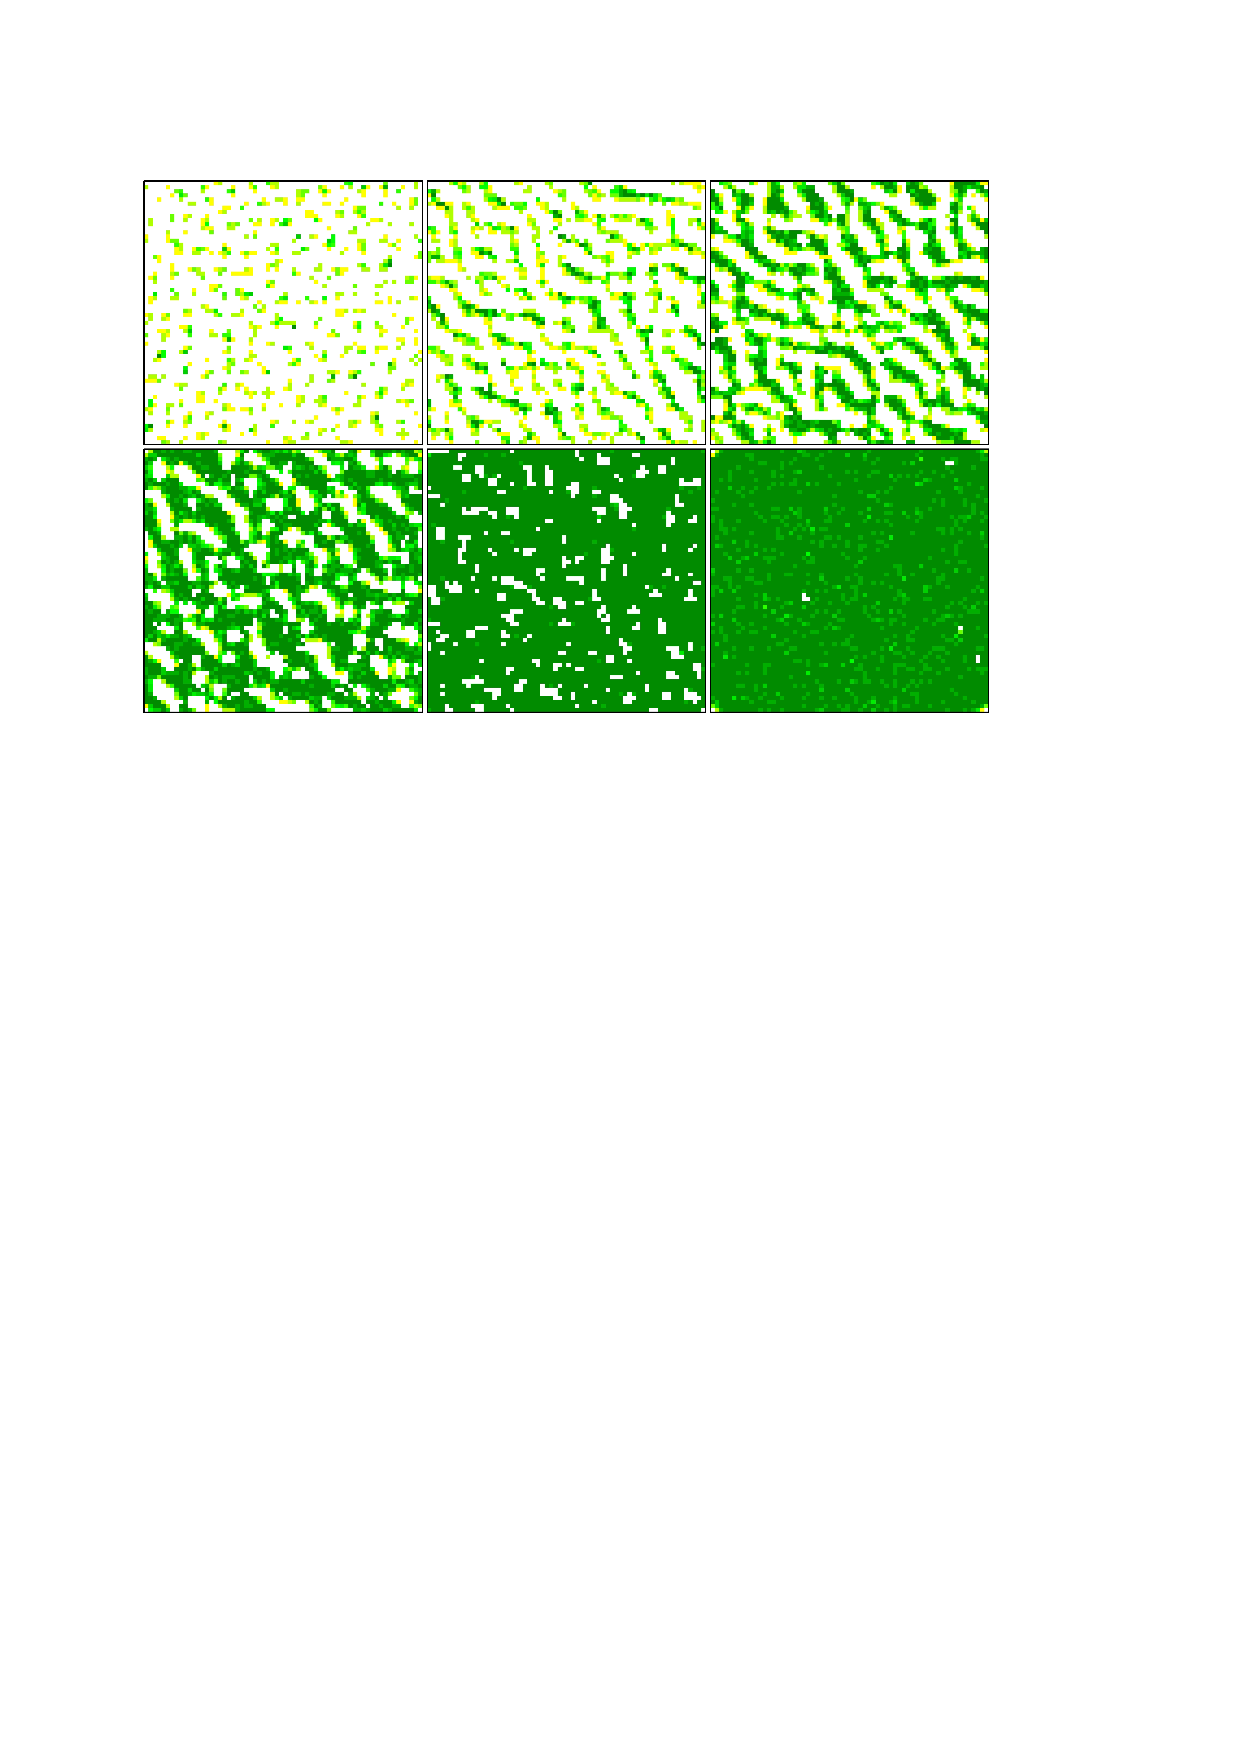
\includegraphics{figures/band_simulation.pdf}}}

\author{Gavan McGrath\\
School of Earth and Environment, The University of Western Australia,\\
M087, 35 Stirling Highway, Crawley, Western Australia, 6009 \and
Christoph Hinz \and Tobias Nanu Frechen\\
Brandenburg University of Technology, Hydrology and Water Resources
Management, \\
Konrad-Wachsmann-Allee 6, 03046 Cottbus, Germany}


\date{DRAFT of \today  , \currenttime}

\maketitle
\thispagestyle{empty}
\pagestyle{empty}

\newpage{}

\cleardoublepage{}

\clearpage{}

\tableofcontents{}

\clearpage{}


\section*{Draft status}
\begin{itemize}
\item Suggestions for overall structuring welcomed!
\item what means Dimensions: {[}:,:{]} ?
\item subroutines and comments on the variables are from file \texttt{coupledModel.f90}
\item \texttt{\textbackslash subroutine\{<name>\}\{<arguments>\}} for displaying a subroutine with its arguments. <name> automatically gets an (emphasized) index entry and a label.
\item \texttt{\textbackslash inout\{<input entries>\}\{<output entries>\}} is for a list of input and output arguments. Missing values get replaced by "no input" or "no output".
\item \texttt{\textbackslash inoutentry[<option>]\{<variableName>\}\{type\}\{dimensions\}\{description\} } for an entry in the input output list. <option> can be empty or "emph" for an emphasized index entry or "none" for no index entry.
\item \texttt{\textbackslash begin\{usessubs\}} is an environment of used subroutines.
\item \texttt{\textbackslash usessubentry\{<subroutineName>\}} is for an entry in the \texttt{usessubs} environment. Entries automatically get an (not emphasized) index entry and a reference to the associated subroutine.
\item I am using the keyword index to index all parameter and variable names.
Good idea? Or shall we make a list with all parameter and variable
names and their description and unit? Like:
\end{itemize}
\begin{table}[H]
\caption{variables}


\begin{tabulary}{\textwidth}{lllllL}
variable &
type &
dimensions &
nom &
unit &
description\tabularnewline
\hline 
\texttt{climParams} &
{[}8-byte real{]} &
{[}4{]} &
 &
 &
climate parameters\tabularnewline
\texttt{infiltParams} &
{[}8-byte real{]} &
{[}6{]} &
 &
 &
vegetation and soil kernel parameters\tabularnewline
\texttt{evapParams} &
{[}8-byte real{]} &
{[}8{]} &
 &
 &
evaporation parameters\tabularnewline
\texttt{discharge} &
{[}integer{]} &
{[}\texttt{m},\texttt{n}{]} &
$Q$ &
$\left[\unitfrac{m^{3}}{S}\right]$ &
discharge\tabularnewline
\texttt{alpha} &
{[}8-byte real{]} &
{[}\texttt{m},\texttt{n}{]} &
$\alpha$ &
 &
\tabularnewline
\end{tabulary}
\end{table}


My suggestion for collaboration: let's use the package "trackchanges".
\annote[Nanu]{Editing}{could look like this} with the following commands:

\texttt{\textbackslash{}add{[}editor{]}\{added text\} }

\texttt{\textbackslash{}remove{[}editor{]}\{removed text\} }

\texttt{\textbackslash{}change{[}editor{]}\{removed text\}\{added
text\} }

\texttt{\textbackslash{}note{[}editor{]}\{note text\} }

\texttt{\textbackslash{}annote{[}editor{]}\{text to annotate\}\{note
text\}}

\clearpage{}

\pagestyle{fancy}
\pagenumbering{arabic}


\section{Introduction}

\section{Theoretical principles}


\subsection{Simulation model}

Runoff, soil moisture storage, transpiration and plant-bare soil transitions
are numerically modeled on a lattice of square cells. The model simulates
the following spatially distributed \index{water balance}water balance:
\begin{equation}
\frac{\partial w_{i}}{\partial t}=P_{i}+R_{i}-Q_{i}-E_{i}-\underset{n}{\sum}T_{n}\label{eq:water-balance}
\end{equation}


\nomenclature[P]{$P$}{precipitation rate in $[\unitfrac{L}{T}]$ (e.g. $\unitfrac{mm}{d}$)}
\nomenclature[R]{$R$}{surface water inflow due to run-on from upslope in $[\unitfrac{L}{T}]$}
\nomenclature[w]{$w$}{local water storage in $[\unit{L}]$}
\nomenclature[t]{$t$}{time in $[\unit{T}]$}
\nomenclature[Q]{$Q$}{surface water discharge as runoff in $[\unitfrac{L}{T}]$}
\nomenclature[E]{$E$}{rate of soil evaporation in $[\unitfrac{L}{T}]$}
\nomenclature[T]{$T$}{transpiration by a plant in $[\unitfrac{L}{T}]$ located at i as well as those in the neghbourhood $(n)$, whose lateral roots extend to that location}


\subsection{Runoff generation}


\subsection{Surface water flow}


\subsection{Short range facilitation}


\subsection{Evaporation and transpiration}


\subsection{Vegetation change}


\subsection{Microtopography}




\section{Application }

\subsection{Build from source}

\subsubsection{Unix Systems}


To use the gfortran compiler execute the following in terminal:

\texttt{gfortran coupledModel.f90}

On Unix systems an \texttt{.out} file is generated. To execute this, type the following into the terminal:

\texttt{./a.out}


\subsection{Installation}


\subsubsection{System requirements}


\subsection{Application prerequisites}


\subsection{Data preperation}


\subsection{Parameterization}


\subsection{Simulation}


\subsection{Output}


\subsection{Appraise and visualize results}


\subsubsection{in R }


\subsubsection{in R and \protect\LaTeX{} (knitr-method)}

\url{http://yihui.name/knitr/}

\subsubsection{in Excel}

\clearpage{}

\section{Implementation}

\subsection{Overview}

\subsection{Implementation strategy}


\subsection{Subroutines}


\subsubsection{Simulation\index{simulation}}

\subroutine{SimCODE}{m, n, mn, simflags, climParams, infiltParams, evapParams,\\ vegParams, erParams, resultsFID}

\inout{
\inoutentry[emph]{m}{integer}{}{number of rows}
\inoutentry{n}{integer}{}{number of colums}
\inoutentry{mn}{integer}{}{$=$ \texttt{m$\cdot$n}}
\inoutentry{simflags}{integer}{6}{{[}1{]} $\ldots$ is for this, {[}2{]} $\ldots$ is for that, \note[Nanu]{should be explained!}}
\inoutentry{climParams}{8-byte real}{4}{\ \annote[Nanu]{climate parameters}{how to input these?}}
\inoutentry{infiltParams}{8-byte real}{6}{\ \remove[Nanu]{vegetation and} soil kernel parameters}
\inoutentry{evapParams}{8-byte real}{8}{evaporation parameters}
\inoutentry{vegParams}{8-byte real}{5}{vegetation \remove[Nanu]{and soil kernel} parameters}
\inoutentry{erParams}{8-byte real}{4}{\ \annote[Nanu]{vegetation and soil kernel parameters}{what specific?}}
\inoutentry{resultsFID}{character}{len=8}{results file id code}
}{
}

\begin{usessubs}
\usessubentry{GD8}
\usessubentry{InfiltProb}
\usessubentry{RoutingWithKernel}
\usessubentry{Erosion}
\usessubentry{Splash}
\usessubentry{Evaporation}
\usessubentry{VegChange}
\end{usessubs}

\subsubsection{Green-ampt infiltration}

\subroutine{GAInfilt}{m, n, dt, inflow, Ksat, wfs, cumInfilt, infex}

\annote[Nanu]{Green-ampt infiltration calculation.}{Literature?}

\inout{
\inoutentry{m,n}{integer}{}{}
\inoutentry{dt}{8-byte real}{}{}
\inoutentry{inflow}{8-byte real}{\mn}{surface runon + precipitation ($R+P$)}
\inoutentry{wfs}{8-byte real}{\mn}{\ \annote[Nanu]{wetting front suction {*} moisture deficit}{formula?}}
\inoutentry{cumInfilt}{8-byte real}{\mn}{\ \annote[Nanu]{cumulative infiltration}{nomenclature?}}
}{
\inoutentry{infex}{8-byte real}{\mn}{infiltration excess}
\inoutentry{cumInfilt}{8-byte real}{\mn}{cumulative infiltration}
}

\subsubsection{\annote[Nanu]{TwoDRandPos}{cannot guess what this means}}

\subroutine{TwoDRandPos}{randOrder, m, n, mn}

\inout{
\inoutentry{m,n}{integer}{}{}
\inoutentry{randOrder}{integer}{\texttt{mn,2}}{}
}{
\inoutentry{randOrder}{integer}{\texttt{mn,2}}{}
}



\begin{usessubs}
\usessubentry{OneDRandList}
\end{usessubs}

\subsubsection{Kinematic wave primer}

\subroutine{KWPrimer}{m, n, topog, manningsN, mask, solOrder, flowdirns,
alpha, deltax,\\ solMax}

Iterate over space to generate calculation a mask. The mask is a 9
x 1 array where 1s indicate that a neighbour (as defined by the position
in mask(x,y) ) discharges to the cell at x,y

\inout{
\inoutentry{m,n}{integer}{}{}
\inoutentry{topog}{integer}{\texttt{mn,n}}{}
\inoutentry{manningsN}{integer}{\texttt{mn,n}}{}
}{
\inoutentry{deltax}{8-byte real}{\mn}{}
\inoutentry{alpha}{8-byte real}{\mn}{}
\inoutentry{solMax}{integer}{}{}
\inoutentry{solOrder}{integer}{\mn}{}
\inoutentry{flowdirns}{integer}{\mn}{flow directions}
\inoutentry{mask}{integer}{\texttt{m},\texttt{n},9}{}
}

\begin{usessubs}
\usessubentry{GD8}
\usessubentry{KMWOrder}
\usessubentry{Neighbours}
\usessubentry{Lookupfdir}
\end{usessubs}

\subsubsection{Kinematic wave\index{kinematic wave}}

\subroutine{KinematicWave}{m, n, ndx, dt, iex, flowdirns, solOrder, solMax,
mask, alpha,\\ deltax, disOld, disNew}

This subroutine calculates the kinematic wave equation for surface
runoff in a network for a single time step. The flow network is given
by the GD8 algorithm calculated on the topography. We assume no interaction
between adjacent flow pathways i.e. water does not overflow in a direction
not specified by the GD8 network. \texttt{iex} is the excess water
from \annote[Nanu]{precip - infiltration + GW discharge}{display as formula?}. 

\[
iex(m,n,1)=qit
\]
\annote[Nanu]{}{should this be displayed as formula or as code?}
\[
iex(m,n,2)=qitPlus
\]


\annote[Nanu]{\texttt{manningsN} the roughness coefficient }{is this in the right place?}

\annote[Nanu]{\texttt{init} a value passed to initialise the variables}{same for this}

\inout{
\inoutentry{m,n}{integer}{}{}
\inoutentry{ndx}{integer}{}{}
\inoutentry{solMax}{integer}{}{}
\inoutentry{flowdirns}{integer}{\mn}{flow directions}
\inoutentry{solOrder}{integer}{\mn}{}
\inoutentry{mask}{integer}{\mn}{}
\inoutentry{alpha}{8-byte real}{\mn}{}
\inoutentry{deltax}{8-byte real}{\mn}{}
\inoutentry{dt}{8-byte real}{}{time step}
\inoutentry{disOld,disNew}{8-byte real}{\mn\texttt{,ndx}}{}
\inoutentry{iex}{8-byte real}{\texttt{m},\texttt{n},2}{}
}{
\inoutentry{disOld, disNew}{8-byte real}{\texttt{m},\texttt{n},\texttt{ndx}}{}
}

\subsubsection{Kinematic wave order}

\subroutine{KMWOrder}{flowdirns, m, n, solutionOrder}

Subroutine assigns values to the matrix \texttt{solutionOrder} to
tell the Kinematic Wave subroutine in which order to solve the KM
equation on the drainage network. Values of 1 assigned to top of catchment,
2 to 1st downstream node etc.. Value at a point is the maximum travel
distance to that point from all points above it.

\inout{
\inoutentry{m,n}{integer}{}{}
\inoutentry{flowdirns}{integer}{\texttt{m},\texttt{n}}{flow directions}
}{
\inoutentry{solutionOrder}{integer}{\texttt{n},\texttt{n}}{}
}

\begin{usessubs}
\usessubentry{Lookupfdir}
\end{usessubs}

\subsubsection{\texttt{OneDRandList(a,mn)}}

\subroutine{OneDRandList}{a, mn}

\inout{
\inoutentry{mn}{integer}{}{}
\inoutentry{a}{integer}{\texttt{mn},2}{}
}{
\inoutentry{a}{integer}{\texttt{mn},2}{}
}

\subsubsection{Lookup for direction}

\subroutine{Lookupfdir}{dirn, dx, dy}

\inout{
\inoutentry{dirn}{integer}{}{}
}{
\inoutentry{dx,dy}{integer}{}{}
}


\subsubsection{Routing with kernel}

\subroutine{RoutingWithKernel}{m, n, mn, precip, infiltKern, storeKern,
newflowdirns,\\ topog, store, discharge, outflow}

\inout{
\inoutentry{m,n}{integer}{}{}
\inoutentry{mn}{integer}{}{}
\inoutentry{infiltKern}{8-byte real}{\mn}{}
\inoutentry{storeKern}{8-byte real}{\mn}{}
\inoutentry{topog}{8-byte real}{\mn}{}
\inoutentry{precip}{integer}{\mn}{}
\inoutentry{store}{integer}{\mn}{}
\inoutentry{newflowdirns}{integer}{\mn}{flow directions}
}{
\inoutentry{outflow}{integer}{}{}
\inoutentry{store}{integer}{\mn}{}
\inoutentry{newflowdirns}{integer}{\mn}{new flow directions}
\inoutentry{discharge}{integer}{\mn}{}
}

\begin{description}
\item [{Notice:}] Periodic boundary conditions can only really be defined
simply for an inclined plane with two adjacent edges defined as the
boundary from which particles are routed to the opposite boundary.
For simplicity it is assumed that the landscape slopes downwards in
the direction of lower x and y.
\end{description}

\begin{usessubs}
\usessubentry{OneDRandList}
\usessubentry{TwoDRandPos}
\usessubentry{Lookupfdir}
\usessubentry{Neighbours}
\usessubentry{fdirLookup}
\end{usessubs}

\subsubsection{Infiltration\index{infiltration} Probability}

\subroutine{InfiltProb}{veg, m, n, K0, ie, rfx, rfy, kf, Kmax, dx, dy, iProb}

This subroutine calculates the spatial distributed infiltration probability.

\inout{
\inoutentry{m,n}{integer}{}{dimensions of the spatial arrays}
\inoutentry{rfx, rfy}{integer}{}{maximum radius for plant effects on soil properties}
\inoutentry{kf}{integer}{}{}
\inoutentry{veg}{integer}{\mn}{vegetation matrix}
\inoutentry{K0}{8-byte real}{}{}
\inoutentry{ie}{8-byte real}{}{}
\inoutentry{Kmax}{8-byte real}{}{}
\inoutentry{dx, dy}{8-byte real}{}{length scales of lattice}
}{
\inoutentry{iProb}{8-byte real}{\mn}{infiltration probability matrix}
}

\subsubsection{List Convolve}

\subroutine{ListConvolve}{base, kernel, convol, m, n, m1, n1}

\inout{
\inoutentry{m,n}{integer}{}{}
\inoutentry{m1,n1}{integer}{}{}
\inoutentry{base}{integer}{\mn}{}
\inoutentry{kernel}{integer}{\texttt{m},\texttt{n}}{}
}{
\inoutentry{convol}{}{\mn}{}
}

\subsubsection{Erosion\index{erosion}}

\subroutine{Erosion}{discharge, topog, newflowdirns, flowResistance, m, n}

\inout{
\inoutentry{m,n}{integer}{}{dimensions of the spatial arrays}
\inoutentry{discharge}{integer}{\mn}{discharge has units of $\unitfrac{mm}{year}$}
\inoutentry{newflowdirns}{integer}{\mn}{new flow directions}
\inoutentry{flowResistance}{8-byte real}{\mn}{flow resistance; effective $d_{40}$ grainsize in $\unit{mm}$}
\inoutentry{topog}{8-byte real}{\mn}{topography}
}{
\inoutentry{topog}{8-byte real}{\mn}{topography}
}

\begin{usessubs}
\usessubentry{Lookupfdir}
\end{usessubs}

\subsubsection{Splash}

\subroutine{Splash}{topog, veg, Dv, Db, m, n}

\inout{
\inoutentry{m,n}{integer}{}{dimensions of the spatial arrays}
\inoutentry{veg}{integer}{\mn}{}
\inoutentry{topog}{8-byte real}{\mn}{topography}
\inoutentry{Dv,Db}{8-byte real}{}{$\unitfrac{m^{2}}{kyr}$}
}{
\inoutentry{topog}{8-byte real}{\mn}{topography}
}

\begin{usessubs}
\usessubentry{Neighbours}
\end{usessubs}

\subsubsection{Find holes}

\subroutine{FindHoles}{newtopog,holes}

\inout{
\inoutentry{newtopog}{8-byte real}{:,:}{topography}
}{
\inoutentry{holes}{8-byte real}{:,:}{}
}

\begin{lstlisting}[caption={a program listing could look like this;
notice the language sensitive formatting},label={lis:a-program-listing},breaklines=true,tabsize=4]
SUBROUTINE FindHoles(newtopog,holes) 
IMPLICIT NONE

REAL*8, DIMENSION(:,:), INTENT(IN) :: newtopog 
INTEGER, INTENT(OUT) :: holes

INTEGER :: m,n,i,j,k,l 
m=SIZE(newtopog,1) 
n=SIZE(newtopog,2)

DO i=2,m-1 
DO j=2,n-1   
    holes=0   
	DO k=-1,1   
	DO l=-1,1     
(*\label{test}*)		IF (newtopog(i,j) < newtopog(i + k, j + l)) THEN
	    	holes = holes + 1     
		END IF   
	END DO   
	END DO   
	IF (holes.ge.8) THEN     
		holes = 1     
		RETURN   
	END IF 
END DO 
END DO

END SUBROUTINE FindHoles
\end{lstlisting}


Listing \ref{lis:a-program-listing} shows, how code can be inserted
into the document. With line numbers and Fortran specific code highlighting. 

It is possible to refer to individual lines inside the listing with
\LaTeX{} commands \texttt{\textbackslash{}label\{\}} and \texttt{\textbackslash{}ref\{\}},
so references get updated if the code changes. For example line \ref{test}
in listing \ref{lis:a-program-listing}, where the first \texttt{IF}-condition
begins.

The code in the listing could be loaded from an external file (for
example the actual Fortran file). 


\subsubsection{Evaporation\index{evaporation}}

\subroutine{Evaporation}{veg, eTActual, bareE, store, tsteps, rcx, rcy, kc, dx, dy, \\ params}

This version cycles through sites and evaporates water from site and
neighbouring sites if vegetated.

\inout{
\inoutentry{veg}{integer}{:,:}{}
\inoutentry{eTActual}{integer}{:,:}{}
\inoutentry{bareE}{integer}{:,:}{}
\inoutentry{store}{integer}{:,:}{}
\inoutentry{tsteps}{integer}{}{}
\inoutentry{rcx, rcy, kc}{8-byte real}{}{}
\inoutentry{dx, dy}{8-byte real}{}{}
\inoutentry{params}{8-byte real}{7}{}
}{
\inoutentry{store}{integer}{:,:}{}
\inoutentry{eTActual}{integer}{:,:}{}
\inoutentry{bareE}{integer}{:,:}{}
}

\begin{usessubs}
\usessubentry{TwoDRandPos}
\end{usessubs}

\subsubsection{Neighbours}

\subroutine{Neighbours}{order, posij, dom, neighbs}

\inout{
\inoutentry{order}{integer}{}{}
\inoutentry{posij}{integer}{2}{}
\inoutentry{dom}{integer}{2}{}
}{
\inoutentry{neighbs}{integer}{\annote[Nanu]{(order*2+1)**2,2}{as formula?}}{}
}

\subsubsection{LSDs}

\subroutine{LSDs}{order, posxy, topog, m, n, lsdList}

This function returns the matrix positions:

\vspace{-2mm}
\begin{description}
\item [{LSD1:}] the position of the neighbouring cell with the steepest
slope downhill
\item [{LSD2:}] the position of the neighbouring cell with second steepest
slope adjacent LSD1
\item [{otherpos:}] the position of the other neighbouring cell the mirror
reflection about LSD1 of LSD2
\end{description}

\inout{
\inoutentry{m,n}{integer}{}{}
\inoutentry{posxy}{integer}{2}{}
\inoutentry{topog}{8-byte real}{\mn}{}
}{
\inoutentry{lsdList}{integer}{3,2}{}
}

\begin{usessubs}
\usessubentry{Neighbours}
\usessubentry{RotateArray}
\end{usessubs}

\subsubsection{Array rotation}

\subroutine{RotateArray}{list, m, n, leftorRight}

\inout{
\inoutentry{m,n}{integer}{}{}
\inoutentry{list}{integer}{\mn}{}
\inoutentry{leftorRight}{integer}{}{}
}{
\inoutentry{list}{integer}{\mn}{}
}

\subsubsection{Pos1D}

\subroutine{Pos1d}{list, m, n, match, rownum}

\inout{
\inoutentry{m,n}{integer}{}{}
\inoutentry{list}{integer}{\mn}{}
\inoutentry{match}{integer}{\texttt{n}}{}
}{
\inoutentry{rownum}{integer}{\texttt{m}}{}
}

\subsubsection{GD8 fow directions}

\subroutine{GD8}{topog, flowdirns, m, n}

\inout{
\inoutentry{m,n}{integer}{}{}
\inoutentry{topog}{8-byte real}{\mn}{}
}{
\inoutentry{flowdirns}{integer}{\mn}{flow directions}
}

\begin{usessubs}
\usessubentry{makeOrds}
\usessubentry{Pos1d}
\usessubentry{endShift}
\usessubentry{LSDs}
\usessubentry{fdirLookup}
\usessubentry{RotateArray}
\end{usessubs}

\subsubsection{New GD8 \index{flow directions}flow directions}

\subroutine{NewGD8}{topog, lakes, flowdirns, m, n}

Calculates flow directions following the \index{GD8-algorithm}GD8-algorithm
of \citet{Paik2008a}

\inout{
\inoutentry{m,n}{integer}{}{}
\inoutentry{lakes}{integer}{\mn}{}
\inoutentry{topog}{8-byte real}{\mn}{}
}{
\inoutentry{flowdirns}{integer}{\mn}{flow directions}
}

\begin{usessubs}
\usessubentry{makeOrds}
\usessubentry{Pos1d}
\usessubentry{endShift}
\usessubentry{LSDs}
\usessubentry{fdirLookup}
\usessubentry{Neighbours}
\end{usessubs}

\subsubsection{\texttt{fdirLookup(dirnxy, idirn)}}
\subroutine{fdirLookup}{dirnxy, idirn}

\inout{
\inoutentry{dirnxy}{integer}{2}{}
}{
\inoutentry{idirn}{integer}{}{}
}

\subsubsection{Array sort}

\subroutine{qsortd}{x, ind, n, incdec}

This subroutine uses an order $n\cdot\log(n)$ quick sort to sort
a real (double precision/8-byte) array $x(n)$ into increasing order.

\inout{
\inoutentry{x(n)}{8-byte real}{}{vector of length \texttt{n} to be sorted}
\inoutentry{n}{integer}{}{length of the array \texttt{x(n)}}
\inoutentry{incdec}{integer}{}{if positive the ind is returned so values decreasing order}
\inoutentry{incdec}{integer}{}{}
}{
\inoutentry{ind(n)}{integer}{}{vector of length $\geqq$ \texttt{n}; sequence of indices $1,\ldots,n$ permuted in the same fashion as x would be: $y(i)=x\left(ind(i)\right)$}
}

\texttt{ind} is initialized to the ordered sequence of indices $1,\ldots,n$,
and all interchanges are applied to \texttt{ind}. \texttt{x} is devided
into two portions by picking a central element $t$. The first and
last elements are compared with $t$, and interchanges are applied
as necessary so that the three values are in ascending order. Interchanges
are then applied so that all elements greater than $t$ are in the
upper portion of the array and all elements less than $t$ are in
the lower portion. The upper and lower indices of one of the portions
are saved in local arrays, and the process is repeated iteratively
on the other portion. When a portion is completely sorted, the process
begins again by retrieving the indices bounding another unsorted portion.

Note: IU and IL must be dimensioned $\geqq\log(n)$ where $\log$
has base 2.

Credit goes to Robert Renka Oak Ridge Natl. Lab.

\subsubsection{endShift}

\subroutine{endShift}{arr, rownum, mn, n}

\inout{
\inoutentry{rown}{integer}{}{}
\inoutentry{n}{integer}{}{}
\inoutentry{mn}{integer}{}{}
\inoutentry{arr}{integer}{mn,n}{}
}{
\inoutentry{arr}{integer}{mn,n}{}
}

\subsubsection{makeOrds}

\subroutine{makeOrds}{topog, ords, m, n}

\inout{
\inoutentry{m,n}{integer}{}{}
\inoutentry{topog}{8-byte real}{\mn}{}
}{
\inoutentry{ords}{integer}{size(topog),2}{}
}

\begin{usessubs}
\usessubentry{qsortd}
\end{usessubs}

\subsubsection{Vegetation Change}

\subroutine{VegChange}{veg, m, n, vegParams, store, actualET, isEmerge, isGrow}

\inout{
\inoutentry{m,n}{integer}{}{}
\inoutentry{isGrow}{integer}{}{}
\inoutentry{isEmerge}{integer}{}{}
\inoutentry{vegParams}{8-byte real}{5}{}
\inoutentry{veg}{integer}{\mn}{}
\inoutentry{store}{integer}{\mn}{}
\inoutentry{actualET}{integer}{\mn}{}
}{
\inoutentry{veg}{integer}{\mn}{}
\inoutentry{store}{integer}{\mn}{}
\inoutentry{actualET}{integer}{\mn}{}
}

\subsection{Customizability}

\clearpage{}

\fancyhead[RE,LO]{}

\settowidth{\nomlabelwidth}{$w$}
\printnomenclature{}

\clearpage{}

\phantomsection\addcontentsline{toc}{section}{List of Figures, Tables and Listings}\listoffigures

\clearpage{}

\listoftables

\clearpage{}

\renewcommand{\rightmark}{LIST OF LISTINGS}
\renewcommand{\lstlistlistingname}{List of Listings}
\lstlistoflistings

\clearpage{}
\renewcommand{\rightmark}{INDEX}

\phantomsection\addcontentsline{toc}{section}{Index}

\printindex{}

\thispagestyle{fancy}

\clearpage{}

\renewcommand{\rightmark}{REFERENCES}
\bibliographystyle{apa}
\phantomsection\addcontentsline{toc}{section}{\refname}\bibliography{GavansDocumentation}

\clearpage{}

\appendix

\section{Appendix}

\end{document}
